\documentclass[14pt]{extarticle}
\usepackage{amsmath}
\usepackage{amssymb}
\usepackage{tikz}
\usetikzlibrary{calc}
%\usetikzlibrary{trees}
\usepackage{hyperref}
\usepackage{graphicx}
\graphicspath{ {../../chap05/} }
\usepackage[top=0.75in, bottom=0.75in, left=0.75in, right=0.75in]{geometry}
\newcommand*{\Scale}[2][4]{\scalebox{#1}{\ensuremath{#2}}}%
\usepackage[shortlabels]{enumitem}
\usepackage[most]{tcolorbox}
\definecolor{bg}{RGB}{255,249,227}
% \usepackage{showframe}
\title{\vspace{-5ex}Math 208 Section 5.2 and 5.3}
\date{\vspace{-10ex}}
\usepackage{multicol}
\setlength{\columnsep}{1cm}
\newcommand{\tikzmark}[1]{\tikz[overlay,remember picture] \node (#1) {};}
\newcommand{\DrawBox}[4][]{%
	\tikz[overlay,remember picture]{%
		\coordinate (TopLeft)     at ($(#2)+(-0.2em,0.9em)$);
		\coordinate (BottomRight) at ($(#3)+(0.2em,-0.3em)$);
		%
		\path (TopLeft); \pgfgetlastxy{\XCoord}{\IgnoreCoord};
		\path (BottomRight); \pgfgetlastxy{\IgnoreCoord}{\YCoord};
		\coordinate (LabelPoint) at ($(\XCoord,\YCoord)!0.5!(BottomRight)$);
		%
		\draw [red,#1] (TopLeft) rectangle (BottomRight);
		\node [below, #1, fill=none, fill opacity=1] at (LabelPoint) {#4};
	}
}
\usepackage{multicol}
\setlength{\columnsep}{1cm}

\begin{document}
\maketitle		
\section*{Homework, Reading, and Other}
\begin{itemize}
	\item Section 5.1
	\item Section 5.2
	\item Section 5.3
\end{itemize}

\section*{Goals}
\begin{itemize}
	\item Using graphs, understand and analyze systems of linear inequalities
	\item Solve for corner points and identify quadrants
	\item Identify bounded and unbounded solution regions
	\item Define and evaluate linear programming terms
	\item Construct a model
	\item Determine optimal solutions from a graph
\end{itemize}

\section*{5.2 Systems of Linear Inequalities in Two Variables}
We learned how to graph a linear inequality. Now we are going to use what we learned to solve systems of linear inequalities. When we solve systems graphically, we graph each inequality in the system. Then the intersection of all of the graphs in the system is the solution region.

\subsection{Examples}
See these \href{https://www.desmos.com/calculator/uvhr3l5lbe}{Desmos graphs for 5.2}
\\\\
Solve graphically \\
\begin{multicols}{3}
	\begin{align*}
		3x + y &\leq 21 \\
		x-2y &\geq 0
	\end{align*}
	\vspace{1.cm}
	\\ 
	\begin{tabular}{c|c}
		x & y \\ \hline
		0 & 21 \\
		7 & 0 \\ \hline
		0 & 0 \\
		2 & 1
	\end{tabular}
	\\
	\begin{tabular}{ccc}
		Test (0,0), & $0 \leq 21$ & is T \\ & & \\
		Test (0,1), & $-2 \geq 0$ & is F
	\end{tabular}
\end{multicols}
\begin{center}
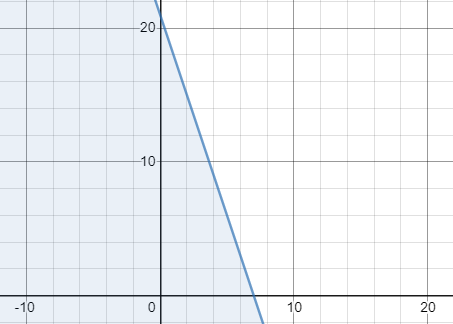
\includegraphics[width=0.48\linewidth]{5-2-1a}
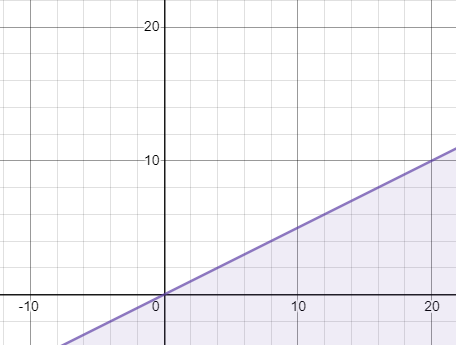
\includegraphics[width=0.46\linewidth]{5-2-1b}
\end{center}
\begin{center}
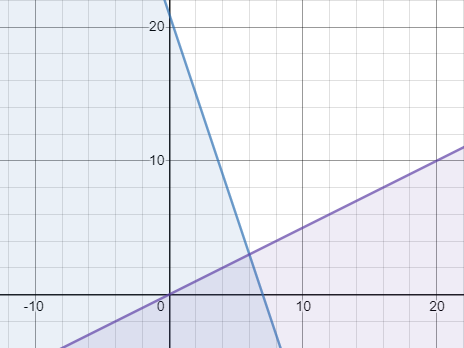
\includegraphics[width=0.9\linewidth]{5-2-1c}
\end{center}
The solution space is unbounded below and it has one corner point at $(6,3)$.
\\\\
Solve graphically \\
\begin{multicols}{3}
	\begin{align*}
		5x + y &\geq 20 \\
		x+y &\leq 12 \\
		x+ 3y &\geq 18 \\
		x &\geq 0 \\
		y &\geq 0
	\end{align*}
	\vspace{1.0cm}
	\\ 
	\begin{tabular}{c|c}
		x & y \\ \hline
		0 & 20 \\
		4 & 0 \\ \hline
		0 & 12 \\
		12 & 0 \\ \hline
		0 & 6 \\
		18 & 0
	\end{tabular}
	\\
	\begin{tabular}{ccc}
		Test (0,0), & $0 \geq 20$ & is F \\ & & \\
		Test (0,0), & $0 \leq 12$ & is T \\ & & \\
		Test (0,0), & $0 \geq 18$ & is F
	\end{tabular}
\end{multicols}
\begin{center}
	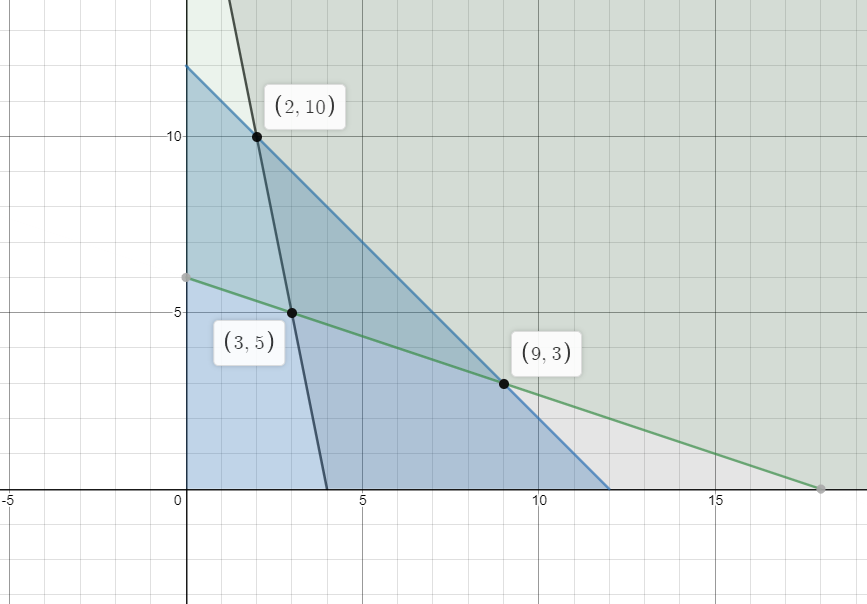
\includegraphics[width=0.9\linewidth]{5-2-2}
\end{center}
The solution space is bounded with corner points $(2,10), (3,5), (9,3)$.

\cleardoublepage
\section*{5.3 Linear Programming}
Linear programming is a mathematical process that helps with decision making. First we build a mathematical model of our problem and then we use our graphical methods to solve it for a best solution.

\begin{itemize}
	\item Linear programming finds the \textit{optimal value} of an \textit{objective function}. The objective function is in the form of $z = ax + by$
	\item The \textit{decision variables}, x and y, are subject to \textit{problem constraints} in the form of linear inequalities. The decision variables are usually subject to \textit{non-negative constraints}, meaning $x \geq 0, y \geq0$.
	\item The points satisfying both the problem constraints and the nonnegative constraints is called the \textit{feasible region} for the problem.
	\item Any point in the feasible region that produces the optimal value of the objective function is called an optimal solution.
\end{itemize}

\begin{tcolorbox}[enhanced jigsaw,colback=bg,boxrule=0pt,arc=0pt]
	\textbf{Fundamental Theorem of Linear Programming}\\
	If the optimal value of the objective function exists, then that value must occur at one or more of the corner points of the feasible region.
\end{tcolorbox}

\begin{tcolorbox}[enhanced jigsaw,colback=bg,boxrule=0pt,arc=0pt]
	\textbf{Theorem 2: Existence of Optimal Solutions}
	\begin{itemize}
		\item If the feasible region for a linear programming problem is bounded, then both the maximum and the minimum value of the objective function always exist.
		\item If the feasible region is unbounded, then only the minimum or maximum value of the objective function exists.
		\item If the feasible region is empty, then neither the maximum value nor the minimum value of the objective function exist.
		\item For an applied problem, interpret the solution.
	\end{itemize}
\end{tcolorbox}

\begin{tcolorbox}[enhanced jigsaw,colback=bg,boxrule=0pt,arc=0pt]
	\textbf{Constructing a Model}
	\begin{enumerate}
		\item Introduce decision variables.
		\item Construct a table summarizing relevant material, relating columns to the decision variables.
		\item Determine the objective and write a linear objective function.
		\item Write problem constraints using linear equations and inequalities.
		\item Write non-negative constraints.
	\end{enumerate}
\end{tcolorbox}

\begin{tcolorbox}[enhanced jigsaw,colback=bg,boxrule=0pt,arc=0pt]
	\textbf{Geometric Method}
	\begin{enumerate}
		\item Graph the feasible region. Then, if an optimal solution 	exists according to Theorem 2, find the coordinates of 	each corner point.
		\item Construct a corner point table listing the value of the objective function at each corner point.
		\item Determine the optimal solution(s) from the table 
	\end{enumerate}
\end{tcolorbox}

\subsection{Examples}
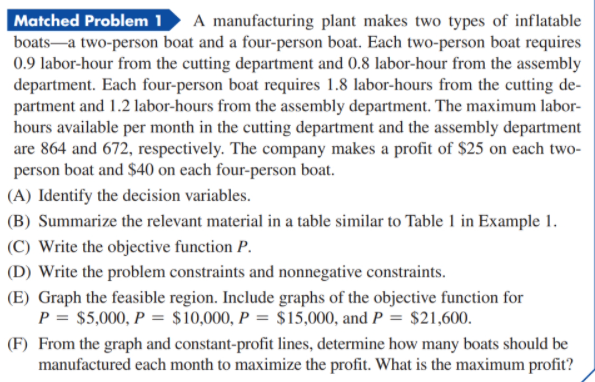
\includegraphics[width=0.85\linewidth]{5-3_04}

\begin{enumerate}[A)]
	\item Decision variables.\\
	$x=$ number of 2-person boats / month \\
	$y=$ number of 4-person boats / month
	\item Table summary \\
	\begin{tabular}{|c|c|c|c|}
		\hline
		& Labor hours & / boat & Labor hours available / month \\
		\hline
		& 2-person & 4-person &  \\
		\hline \hline
		Cutting & 0.9 & 1.8 & 864 \\
		\hline
		Assembly & 0.8 & 1.2 & 672 \\
		\hline \hline
		Profit / boat & \$25 & \$40 &  \\
		\hline
	\end{tabular}
	\item Objective function P. \\
	$P = 25x + 40y$
	\item Constraints
	\begin{align*}
		0.9x + 18y &\leq 864 \\
		0.8x + 1.2y &\leq 672 \\
		x,y &\geq 0
	\end{align*}
	\item Graph
	\begin{center}
		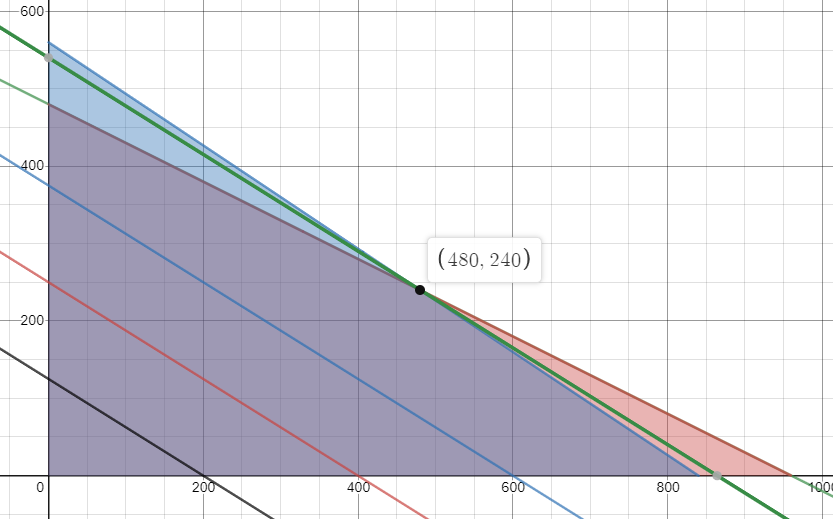
\includegraphics[width=0.9\linewidth]{5-3-p1}
	\end{center}
	\item Maximize profit at $x=480, y=240$, then $P=\$21,600$.
\end{enumerate}

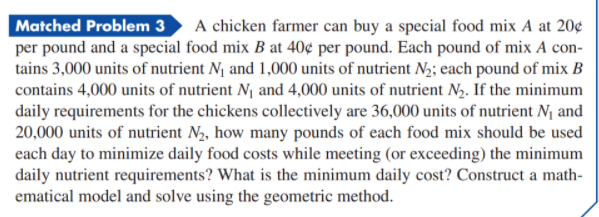
\includegraphics[width=0.9\linewidth]{5-3_03}
\begin{center}
	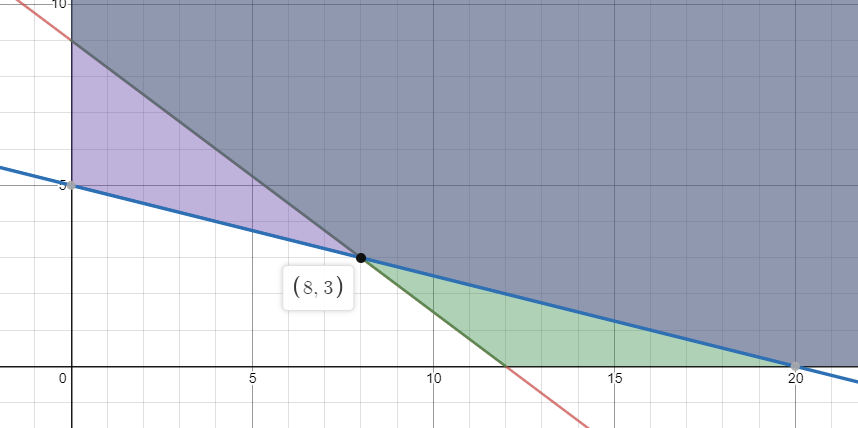
\includegraphics[width=0.9\linewidth]{5-3-p2}
\end{center}

\begin{center}
	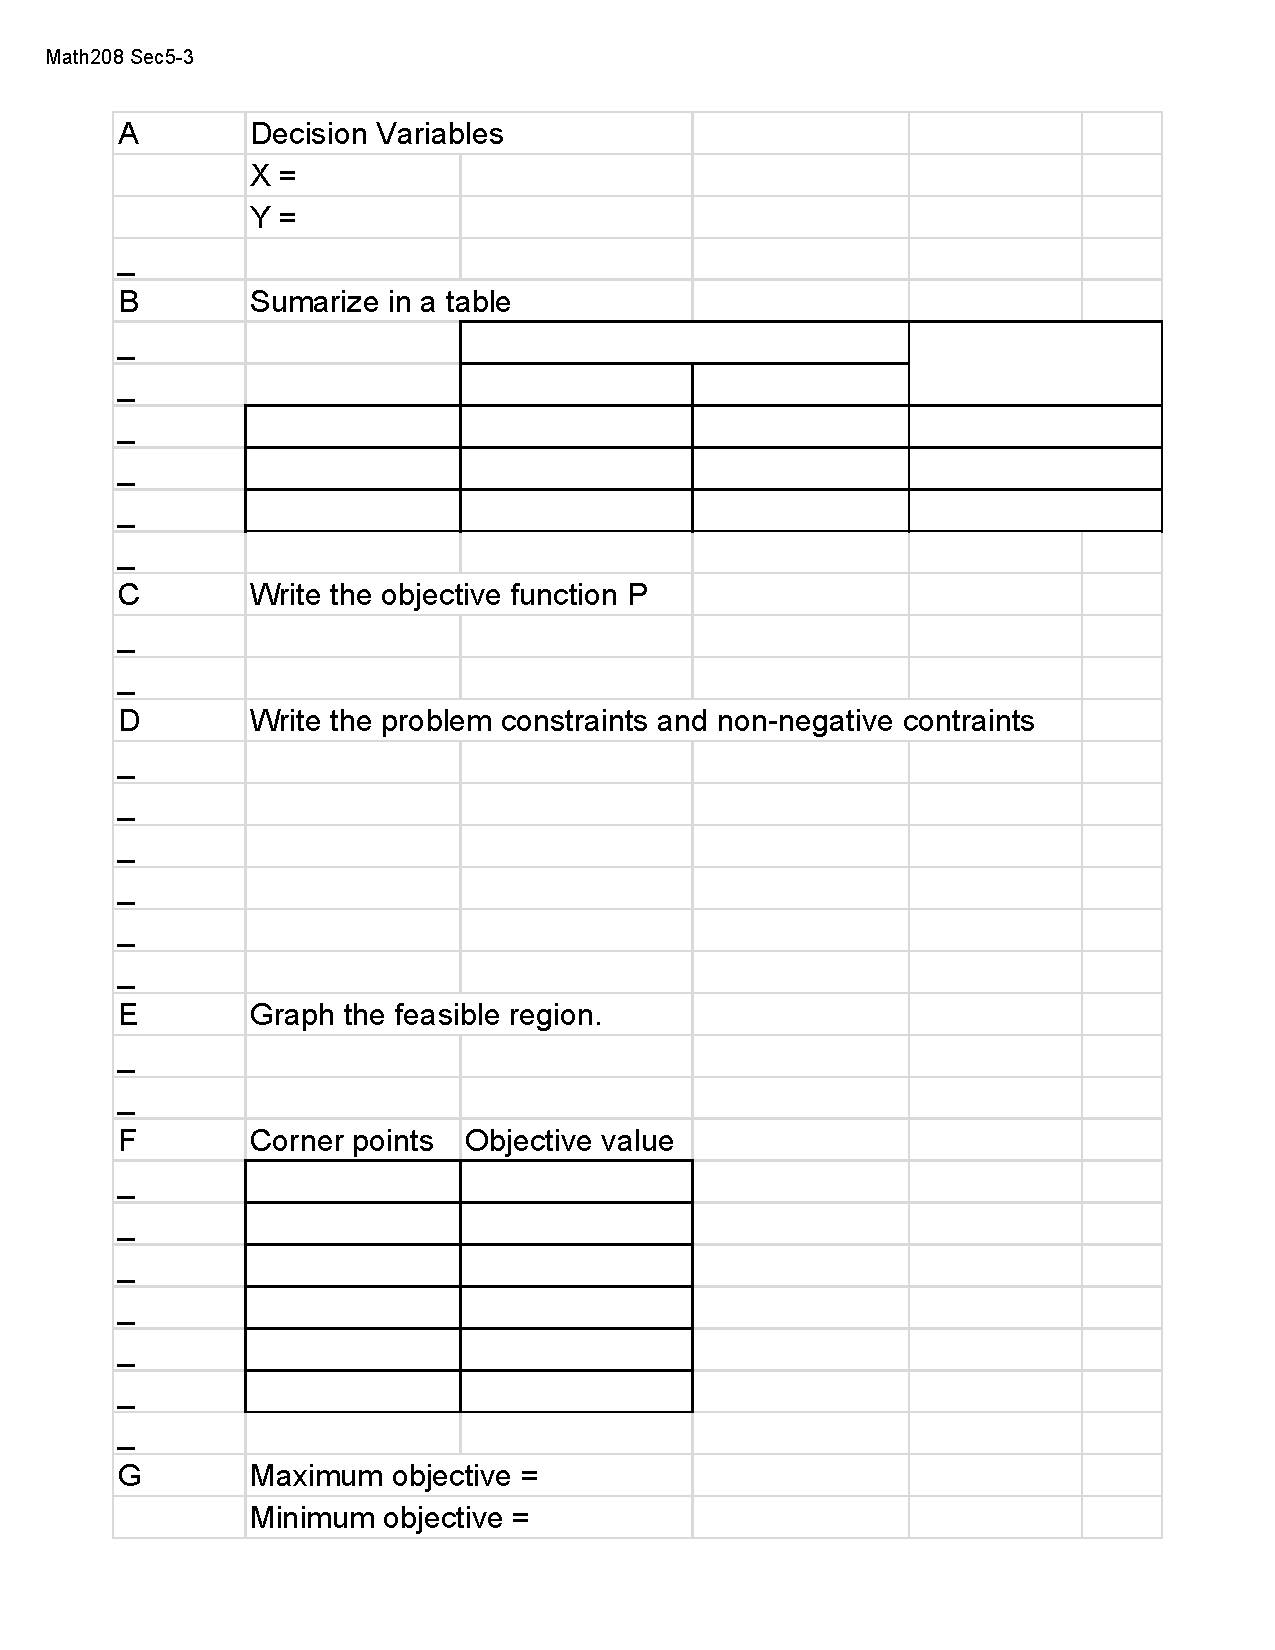
\includegraphics[width=1.0\linewidth]{Math208 Sec5-3 prob2}
\end{center}

\begin{center}
	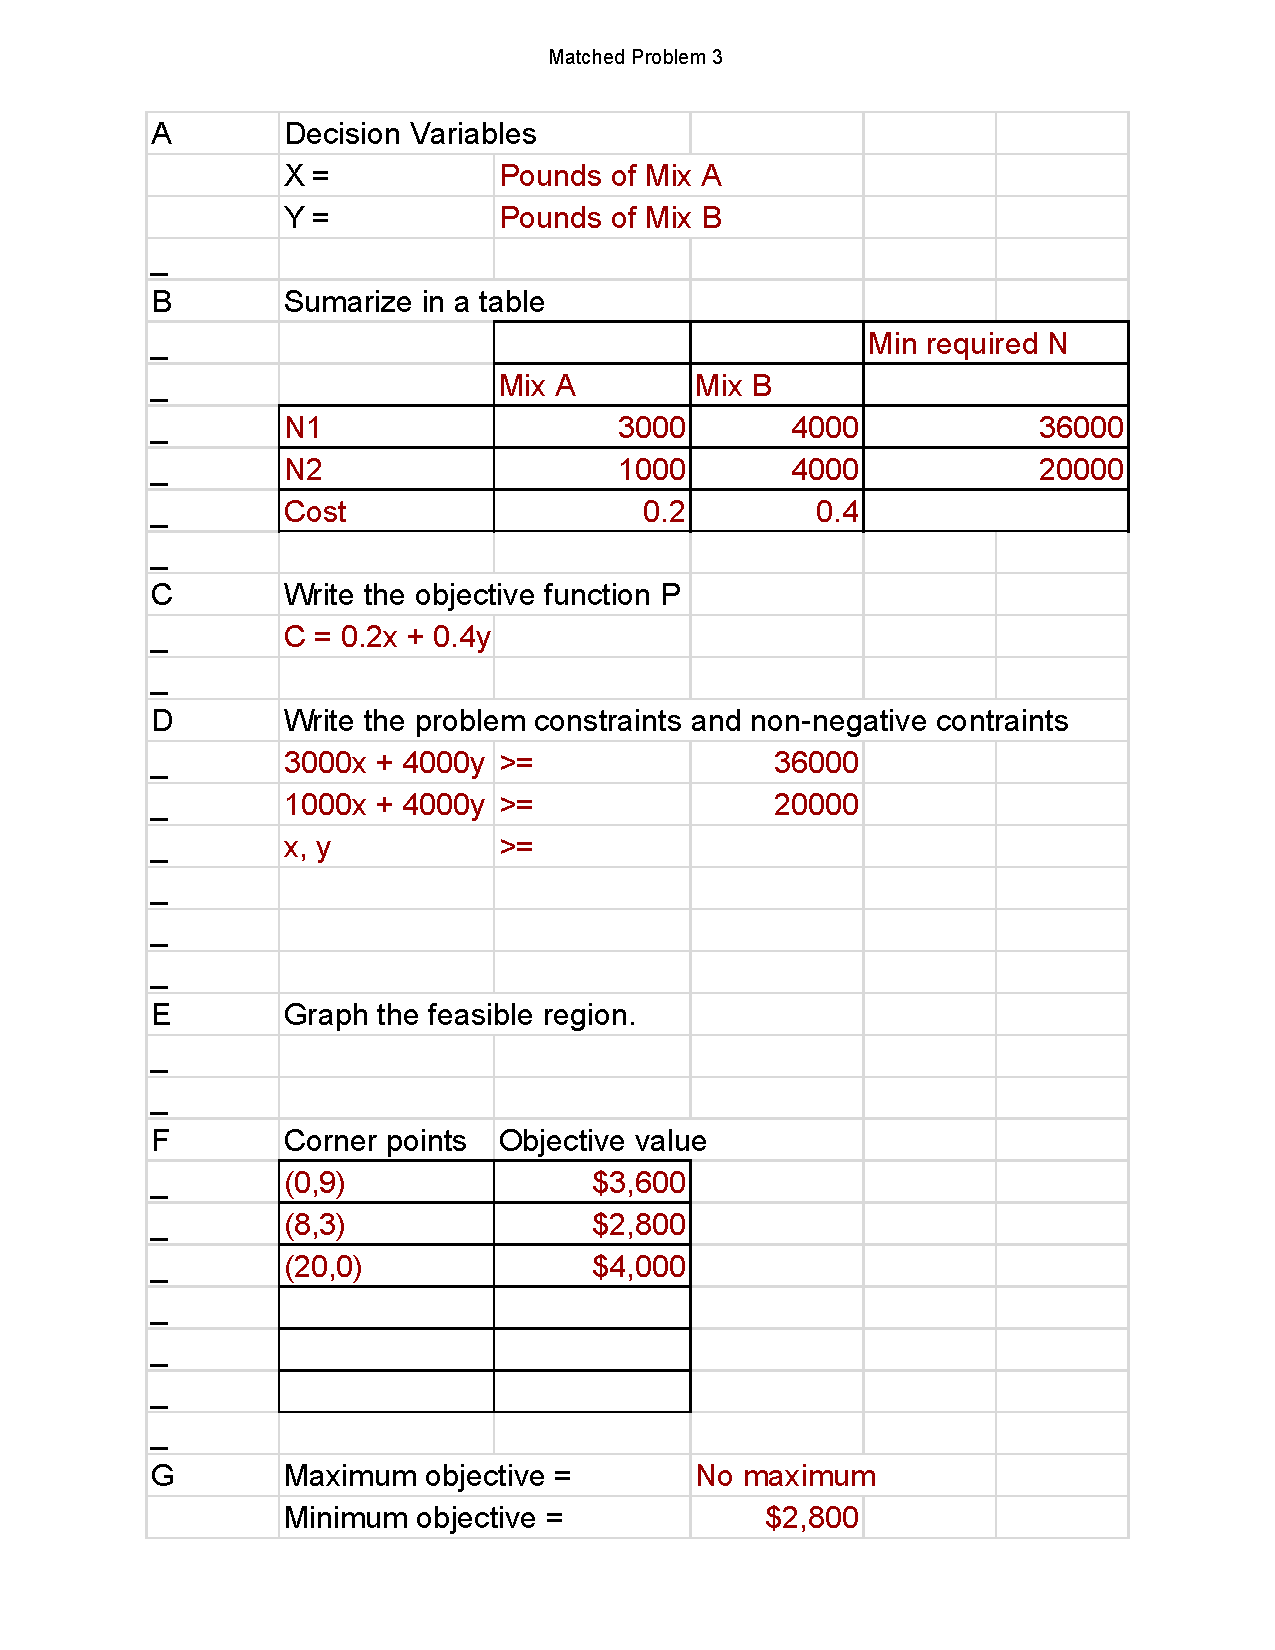
\includegraphics[width=0.9\linewidth]{Math208 Sec5-3 - Sheet3.pdf}
\end{center}


\noindent\rule{\textwidth}{1pt}
{\footnotesize Copyright (C) 2021 Garold Dalton --- Released under GNU General Public License v3.0}


\cleardoublepage


\end{document}
